\documentclass[10pt,a4paper]{book}
\usepackage[utf8]{inputenc}
\usepackage[english]{babel}
\usepackage{amsmath}
\usepackage{amsfonts}
\usepackage{amssymb}
\usepackage{wrapfig}
\usepackage{mathtools}
\usepackage{mathrsfs}
\usepackage[makeroom]{cancel}
\usepackage{graphicx}
\usepackage{cancel}
\usepackage[left=2cm,right=2cm,top=2cm,bottom=2cm]{geometry}
\usepackage{physics}
\usepackage{multicol}
\usepackage{caption}
\usepackage{subcaption}
\usepackage{stmaryrd}
\usepackage{braket} %\braket{a|b|c..}

%main sets:
\newcommand{\Z}{\mathbb{Z}}
\newcommand{\Q}{\mathbb{Q}}
\newcommand{\R}{\mathbb{R}}
\newcommand{\C}{\mathbb{C}}

%math shortcuts
\newcommand{\p}{\partial}
\newcommand{\w}{\omega}
\newcommand{\tf}{\text{TF}}



\author{Alessandro Pacco}
\title{Statistical physics solutions}
\begin{document} 
\maketitle

\chapter*{Chapter 3}
\section*{3.12}

\subsection*{1)}
Since we have periodic conditions the system in $d=1$ is equivalent to having a circle where the spins are placed and where they interact only between neighbors, so that we have $N$ interactions. In $d=2$ we have that the system is equivalent to a square lattice in which every spin has 4 neighbors, so that there are $4N/2=2N$ interactions.
Now we have that
$$Z=\sum_{\{\sigma_i\}}e^{-\beta H}=\sum_{\{\sigma_i\}}e^{K\sum_{\langle i,j\rangle} \sigma_i\sigma_j}=\sum_{\{\sigma_i\}}\prod_{\langle i,j\rangle}e^{K\sigma_i\sigma_j}
$$
Now since you are too stupid to come up with any idea, look at the result of the question and magically find that, since $\sigma_i\sigma_j=\pm 1$, you can write 
$$(1+\sigma_i\sigma_j\tanh K)\cosh K=\frac{\sigma_i\sigma_j(e^K-e^{-K})+(e^K+e^{-K})}{2}=\frac{e^K(\sigma_i\sigma_j+1)+e^{-K}(1-\sigma_i\sigma_j)}{2}=e^{K\sigma_i\sigma_j}$$
Hence recalling that there are $dN$ couples of interactions:
\begin{align*}
Z=\sum_{\{\sigma_i\}}\prod_{\langle i,j\rangle}\cosh K(1+\sigma_i\sigma_j\tanh K)=2^N(\cosh K)^{dN}Q(\tanh K)
\end{align*}


\subsection*{2)}
\subsubsection*{a)}
Notice that when we expand the product $\prod_{\langle i,j\rangle}(1+x\sigma_i\sigma_j)$ then each power of $x$ will have a certain coefficient of the type $\sigma_1^{n_1}\cdots \sigma_N^{n_N}$. Then notice that when we do the summation $\sum_{\{\sigma_i\}}$ then if $\sigma_1^{n_1}\cdots \sigma_N^{n_N}$ contains one of the $n_i$ which is odd, then after the summation the total contribution is gonna be zero. Indeed if wlog $n_1$ is odd, then for each configuration of the $\sigma_2,\ldots,\sigma_N$, we can pick $\sigma_1^{n_1}=\pm 1$ and the sum disappears. Hence the only possible configurations that have all the spins appearing with even exponents are the null configuration (all exponents are zero) and the complete configuration (all exponents are 2). 

\subsubsection*{b)}
Then we get that 
$$Z=(\cosh K)^N \sum_{\{\sigma_i\}} \bigg(1+(\tanh K)^N\sigma_1^{2}\ldots\sigma_N^2\bigg)=2^{N}(\cosh K)^N(1+(\tanh K)^N)$$

\subsubsection*{c)}
We have that
\begin{align*}
\langle \sigma_a\sigma_{a+r}\rangle =\frac{(\cosh K)^N}{Z}\sum_{\{\sigma_i\}}\bigg(\sigma_a\sigma_{a+r}\prod_{\langle i,j\rangle}(1+\sigma_i\sigma_j\tanh K)\bigg)
\end{align*}
Then we have that if we expand inside with powers of $\tanh K$ we need to compute which configurations of the $\sigma_i^{n_i}$ will not add up to zero once summed over $\sum_{\{\sigma_i\}}$. The only two configurations are those connecting $\sigma_a$ and $\sigma_{a+r}$, i.e. $\sigma_a\sigma_{a+1}^2\ldots\sigma_{a+r-1}^2\sigma_{a+r}$ and $\sigma_{a+r}\sigma_{a+r+1}^2\ldots\sigma_N^2\ldots\sigma_{a-1}^2\sigma_a$. Hence we finally get 
\begin{align*}
\langle \sigma_a\sigma_{a+r}\rangle&=\frac{(\cosh K)^N}{Z}\sum_{\{\sigma_i\}}\bigg((\tanh K)^{r}+(\tanh K)^{N-r}\bigg)=\frac{(\cosh K)^N}{Z}2^N\bigg((\tanh K)^{r}+(\tanh K)^{N-r}\bigg)\\
&=\frac{(\tanh K)^r+(\tanh K)^{N-r}}{1+(\tanh K)^N}
\end{align*}


\subsection*{3)}
\subsubsection*{a)}
Like before we need to take into account all those configurations of the $\sigma_1^{n_1}\ldots\sigma_N^{n_N}$ such that their exponents are even, and hence they don't cancel out when summing over all the possible configurations. If we see the spin system as a graph where every spin has exactly 4 connections, then a configuration that doesn't cancel is such that any involved spin has an even number of links activated. For $\tanh k$ with powers of $1,2,3$ there is nothing appearing, since we need to pass though every involved spin at least two times (or 4 ), which is clearly impossible. So the first term is $(\tanh K)^4$ , which is given by the squares (so in total $N$ of them). Then there is the term in $(\tanh K)^6$, which is made of rectangles of one side of 1 link and one side of 2 links: in total $12N/6=2N$. For $(\tanh K)^8$ we have either rectangles of one side made of 1 link and the other made of 3 or squares of side 2 or the little $L$ made of three squares attached and linked on the boundary or two one sided different squares: in total $N+2N+4N+N(N-5)/2$
where the first two are trivial, the third one is found by thinking that there is a bijection between taking a square of side one and taking 4 $L$ that with it form a 2 sided square, the fourth one is found by saying that for any chosen square I can choose other $(N-5)$, so that we have a total of $N(N-5)/2$.
Finally 
$$Q=1+N(\tanh K)^4+2N(\tanh K)^6+\frac{N}{2}(N+9)(\tanh K)^8 +o((\tanh k)^8)$$

\subsubsection*{b)}
Recall that the expansion of $\ln(x)$ for $x$ close to $0$ is $\ln(1+x)=x-x^2/2$
\begin{align*}
F&=-k_BT\log(Z)
=-k_BT\bigg(N\log(2)+2N\log(\cosh K)+\log(Q)\bigg)\\
&=-k_BNT\bigg(\log(2)+2\log(\cosh K)+(\tanh K)^4+2(\tanh K)^6+\frac{N+9}{2}(\tanh K)^8-\frac{N}{2}(\tanh K)^8 +o((\tanh k)^8)\bigg)\\
&=-Nk_BT\bigg(\log(2)+2\log(\cosh K)+(\tanh K)^4+2(\tanh K)^6+\frac{9}{2}(\tanh K)^8+o((\tanh k)^8)\bigg)
\end{align*}

It is clearly extensive
\subsubsection*{c)}

The fundamental state is when all the spins are aligned, so that the degeneracy is 2. The energy is $E_0=-2NJ$. 

\subsubsection*{d)}
The first excited state corresponds to having only one spin which is not aligned. Hence we have $g_1=2N$ . Then the energy is $E_1=E_0+8J$, so $\epsilon_1=8J$. The second energy is given by 2 non-aligned neighboring spins:
$\epsilon_2=2(6J)=12J$ and $g_2=2(2N)$ (2 times the number of neghboring spins we can choose). For the third state we have that it can be obtained by three non-aligned neighboring spins, or two non-aligned non-neighboring spins, or 4 non-aligned spins forming a one sided square. Hence we have $\epsilon_3=2(8)J=16J$ and $g_3=2((4N+2N)+N+N(N-5)/2))=$
where there are $4N+2N$ ways to choose 3 neighboring spins, $N$ ways to choose a square and $N(N-5)/2$ ways to choose two non-neighboring spins.

\subsubsection*{e)}








\chapter*{Chapter 6}


\section*{6.1}
\subsection*{1)}
The derivative of $\mathscr{V}$ is 
$$\frac{d\mathscr{V}}{dt}=\sum_i\dot{\mathbf{p}}_i\cdot \mathbf{r}_i+\mathbf{p}_i\cdot\dot{\mathbf{r}}_i=\sum_i\mathbf{F}_i\cdot \mathbf{r}_i+\frac{\mathbf{p}_i^2}{m}=\mathscr{H}+2E_c$$

then  if we take the average we have that
$$\overline{\frac{d\mathscr{V}}{dt}}=\frac{d\overline{\mathscr{V}}}{dt}=\frac{d}{dt}\bigg(\lim_{T\to\infty}\sum_i\frac{1}{T}\int_0^T\frac{1}{2m}\frac{d\mathbf{r}_i^2}{dt}\bigg)=\frac{d}{dt}\bigg(\sum_i\lim_{T\to\infty}\frac{\mathbf{r}_i^2(T)-\mathbf{r}_i(0)}{2mT}\bigg)=0$$
where we used that since the volume $V$ is finite, then the position of a particle is bounded. Hence it follows that 
$$\overline{\mathscr{H}}=-2\overline{E_c}$$

\subsection*{2)}

We decompose a force $\mathbf{F}_i$ as $\mathbf{F}_{int}-P(\vec{S}_1+\cdots+\vec{S}_6)=\mathbf{F}_{int}+\mathbf{F}_{ext}$ where we took into account the 6 oriented faces of the box where the particles are contained. Then we have
$$\overline{\sum_i\mathbf{F}_{ext}\cdot\mathbf{r}_i}=-6PS\bigg(\overline{\sum_i \mathbf{n}\cdot \mathbf{r}_i}\bigg)$$
where we said that all the 6 faces will give the same contribution ($S$ is the surface of a face), and $\mathbf{n}$ is just one of the 6 unitary vectors giving theh orientation of a face.
Then 
$$-6PS\bigg(\overline{\sum_i \mathbf{n}\cdot \mathbf{r}_i}\bigg)=-6PS\frac{d}{2}=-3PV$$
where $d$ is the length of a side of the cube and where we used that the average of the sum of the projections of the vectors of each particle on one surface is going to be at the middle, i.e. at $d/2$.

\subsection*{3)}











\section*{6.3}




Remark: diffraction and diffusion.

Send a laser on a lens $D1$. We have $A(x)=0$ if the light doens't pass, 1 otherwise. Introduce the angle $\theta$. Then $r(x,z)\approx r_0(z)-x\sin(\theta)$. This approximation is valid only if $x<<d$. The spherical wave coming out of a hole is $E(r)=\frac{E_0}{r}e^{i\frac{2\pi}{\lambda}(r-ct)}$. Then $$E_{tot}(z)=\int dxA(x)\frac{E_0}{r(x,z)}e^{i\frac{2\pi}{\lambda}r(x,z)}\underset{\underset{\text{varie lentement}}{x\to x}}{\approx} \frac{E_0}{r_0(z)}e^{i\frac{2\pi}{\lambda}r_0(z)}\int dxA(x)e^{i2\pi\frac{\sin\theta}{\lambda}x}=\frac{E_0}{r_0(z)}e^{i\frac{2\pi}{\lambda}r_0(z)}TF(A)\frac{\sin\theta}{\lambda}$$
if we mesure the light on the screen, we get that
$$I(z)=|E_{tot}(z)|^2\approx |TF(A)|^2\approx |S|^2$$.



\subsection*{1)}
The potential energy is
$$E_p(\{\vec{r}_i\})=\sum_{i<j}U(|\vec{r}_i-\vec{r}_j|)$$
\subsection*{2)}
The kinetic energy is 
$$E_c=\sum_i \frac{p_i^2}{2m}$$

\subsection*{3)}
The canonical partition function is written as
\begin{align*}
Z&=\frac{1}{N!h^{3N}}\int \prod d^3r_id^3p_i e^{-\beta(\sum_{i<j}U(|\vec{r}_i-\vec{r}_j|)+\sum_i \frac{p_i^2}{2m})}=\frac{1}{N!h^{3N}}\bigg(\sqrt{\frac{2m\pi}{\beta}}\bigg)^{3N}Q_N\\
&=\frac{1}{\lambda^{3N}N!}Q_N
\end{align*}

we know that $\lambda$ is the De Broglie wavelenght, and it is the threshold at which we go to the quantum regime. This meas thatto have a classical desscription the average particle distance has to be $>>\lambda$. Instead when the interparticle distance is smaller than the De Broglie wavelength, then we will need a quantum description.


\subsection*{4)}
The classical description is valid when the average interparticle distance $(V/N)^{1/3}>>\lambda$. Hence $n^{-1/3}>>\lambda$. 

\subsection*{5)}
We have 
$$\rho^{(l)}(\mathbf{x}_1,\cdots,\mathbf{x}_l)=\sum_{i_1\neq \ldots\neq i_l}\langle \delta^{(3)}(\mathbf{x}_1-\mathbf{x}_{i_1})\ldots\delta^{(3)}(\mathbf{x}_l-\mathbf{x}_{i_l})\rangle=\sum_{i_1\neq\ldots\neq i_l}\mathbb{P}(\{\mathbf{x}_1=\mathbf{x}_{i_1}\}\cap \ldots\cap\{\mathbf{x}_l=\mathbf{x}_{i_l}\})$$
where the sum is done over all the positions $\mathbf{x}_{i_1}\ldots\mathbf{x}_{i_l}$ which are taken between the positions of the particles. Hence for $l=2$ we have that 
$$\rho^{(2)}(\mathbf{x},\mathbf{y})d\mathbf{x}d\mathbf{y}\sim \mathbb{P}(\text{1 particle at }\mathbf{x}\pm d\mathbf{x}\cap \text{1 particle at }\mathbf{y}\pm d\mathbf{y})$$
Then we have that 
$$\int d\mathbf{x}d\mathbf{y}\rho^{(2)}(\mathbf{x},\mathbf{y})=\sum_{i_1\neq i_2}\int d\mathbf{x}d\mathbf{y}\mathbb{P}(\{\mathbf{x}=\mathbf{x}_{i_1}\}\cap\{\mathbf{y}=\mathbf{x}_{i_2}\})=\sum_{i_1\neq i_2} 1=N(N-1)\approx N^2$$
and owing to the normalization of $\mathbb{P}(\text{1 particle at }\mathbf{x}\pm d\mathbf{x}\cap \text{1 particle at }\mathbf{y}\pm d\mathbf{y})$, we get that
$$\rho^{(2)}(\mathbf{x},\mathbf{y})d\mathbf{x} d\mathbf{y}=N^2 \mathbb{P}(\text{1 particle at }\mathbf{x}\pm d\mathbf{x}\cap \text{1 particle at }\mathbf{y}\pm d\mathbf{y})$$
therefore now we have that
\begin{align*}
\mathbb{P}(\text{1 particle at }\mathbf{y}\pm d\mathbf{y}|\text{1 particle at }\mathbf{x}\pm d\mathbf{x})&=\frac{\mathbb{P}(\text{1 particle at }\mathbf{y}\pm d\mathbf{y}\cap \text{1 particle at }\mathbf{x}\pm d\mathbf{x})}{\mathbb{P}(\text{1 particle at }\mathbf{x}\pm d\mathbf{x})}\\
&=\frac{\frac{1}{N^2}\rho^{(2)}(\mathbf{x},\mathbf{y})d\mathbf{x}d\mathbf{y}}{\frac{d^3\vec{r}}{V}}=\frac{\frac{1}{N^2}\rho^{(2)}(\mathbf{x},\mathbf{y})d^3\vec{r}d^3\vec{r}}{\frac{d^3\vec{r}}{V}}\\
&=\frac{n^{-2}}{V}\rho^{(2)}(\vec{r})d^3\vec{r}=\frac{1}{V}g(\vec{r})d^3\vec{r}
\end{align*}

where we replaced $\vec{r}=\mathbf{x}-\mathbf{y}$ and we think of it as being $\mathbf{x}=0$. Hence $\frac{1}{V}g(\vec{r})d^3\vec{r}$ is the probability to find a particle at position $\vec{r}\pm d\vec{r}$ knowing that we have a particle at $\vec{0}\pm d\vec{r}$. 

For a perfect gas we have 
$\frac{1}{V}g(\vec{r})d^3\vec{r}=\frac{d^{3}\vec{r}}{V}\Rightarrow g(\vec{r})=1$.



\subsection*{6)}
Benzene is non-polar, hence it is better than water for the diffraction. Difficulty to obtain some data for small $\vec{r}$? If $\vec{ r}$ is too small with respect to the wavelength we don't get diffraction.\\
Estimation of the diamater:
to estimate it pick the value for which thefunction $g(r)=1$,i.e. the value of $r$ for which we have exactly one particle at close distance, and that will give us the typical diameter of a particle. From the figure it is $\sigma\approx 5\cdot 10^{2}nm$.



\subsection*{7)}
Diffraction of a laser beam on the liquid. For diffraction we need that the $\sigma$ is almost the same as the wavelenght of the incoming light. Hence we have resolution$\sim\sigma\sim 500nm$ since we want $\lambda\sim\sigma$. Hence we need a laser of $\lambda \sim 514  nm$.


\subsection*{8)}

$$n=\frac{N}{V}=\frac{N}{M}\frac{M}{V}=\frac{\rho}{m}=\frac{5,39\cdot 10^{-2}}{8\cdot 10^{-15}}\approx 10^{19}m^{-3}$$
minimal volume $\sim\sigma^3$.
We have that
$$n\sigma^3=10^{19}(5\cdot 10^{-7})^3=125\cdot 10^{19-21}\approx 1.25\text{ particles/elementar volume}$$
Hence it is not at all dilute, but mainly dense.

\subsection*{9)}

We work on the LHS:

\begin{align*}
\rho^{(2)}(\vec{x},\vec{y})=\sum_{i_1\neq i_2}
<\delta(\vec{r}_{i_1}-\vec{x})\delta(\vec{r}_{i_2}-\vec{y})>
&=\frac{1}{N!Z}\int\bigg(\prod_{i=1}^N\frac{d\vec{r}_i d\vec{p}_i}{h^3}e^{-\beta H}
\cdot \sum_{i_1\neq i_2}
\delta(\vec{r}_{i_1}-\vec{x})\delta(\vec{r}_{i_2}-\vec{y})\bigg)\\ 
&\underset{Q3}{=}\frac{1}{Q_N}\sum_{i_1\neq i_2}\int\prod_{i=1}^N d^3\vec{r}_i e^{-\beta E_p\{r_i\}}
\delta(\vec{r}_{i_1}-\vec{x})\delta(\vec{r}_{i_2}-\vec{y})\\
&=
\frac{1}{Q_N}N(N-1)\int\prod_{i=1}^N d^3\vec{r}_i
e^{-\beta\sum_{i<j}U(r_i-r_j)}\delta(\vec{r}_1-\vec{x})\delta(\vec{r}_2-\vec{y})\\
&=\frac{N(N-1)}{Q_N}
\int\prod_{i=3}^Nd^3\vec{r}_i
e^{-\beta\big[U(x-y)+\sum_{i=3}^N(U(x-r_i)+U(y-r_i))+\sum_{i>j=3}^N U(r_i-r_j)\big]}
\end{align*}

Now we attack the gradient 

\begin{align*}
\vec{\nabla}_{\vec{x}}\rho^{(2)}(x,y)&=
\frac{N(N-1)}{Q_N}\int\bigg(\prod_{i=3}^Nd^3\vec{r}_i\big[-\beta\nabla U(x-y)-\beta\sum_{i=3}^N\nabla U(x-r_i)\big]\cdot e^{-\beta E_p}\bigg)\\
&=\frac{N(N-1)}{Q_N}(-\beta\nabla U(x-y))\int\prod_{i=3}^Nd^3r_ie^{-\beta E_p}-\frac{N(N-1)}{Q_N}\beta\int\bigg(\prod_{i=3}^Nd^3r_i\big[\sum_{i=3}^N\nabla U(x-r_i)\big]e^{-\beta E_p}\bigg)
\end{align*}

Then we introduce $\sum_{i=3}^Nf(r_i)=\int dzf(z)\sum_{i=3}^N\delta(z-r_i)$. With that decomposition we get

\begin{align*}
\vec{\nabla}_{\vec{x}}\rho^{(2)}(x,y)&=-\beta(\nabla U(x-y))\rho^{(2)}(x,y)-\beta\int \bigg(d^3z\nabla U(x-z)\sum_{i=3}^N\delta^{(3)}(r_i-z)\frac{N(N-1)}{Q_N}\int \prod_{i=3}^Ndr_ie^{-\beta E_p(x,y,r_{i>3})}\bigg)\\
&=-\beta\nabla U(x-y)\rho^{(2)}(x,y)-\beta\int d^3z\nabla U(x-z)\rho^{(3)}(x,y,z)
\end{align*}

where $<>$ is the canonical average.

\subsection*{10)}
Born-Green is general.

$\nabla\rho^{(2)}\approx f(\rho^{(2)},\rho^{(3)})$ and $\nabla \rho^3=f(\rho^{(3)},\rho^{(4)})$, it doens't stop. 

$$\rho^{(l)}(\vec{x}_1,\vec{x}_2,..,\vec{x}_l)=\sum_{i_1\neq..\neq i_l}<\delta(\vec{x}_{i_1}-\vec{x}_{1})..\delta(\vec{x}_{i_l}-\vec{x}_l)>\underset{dilute}{\approx}\sum<\delta(\vec{x}_{i_1}-\vec{x}_{i_1})..\delta(..)>\approx n\sigma^3)^l$$
In practice, if we suppose dilute then $n\sigma^3<<1$ implies that $\rho^{(1)}>>\rho^{(2)}>>...$.

In our case we have 

$$merda da fare$$

By symmetry $\rho^{(2)}(x,y)=\rho^{(2)}(x-y)=\rho^{(2)}(r)$. If we rewrite Born-Green at order 2 we get

$$\frac{d}{dr}\rho^{(2)}=-\beta(\frac{d}{dr}U(r))\rho^{(2)}(r)\Rightarrow \rho^{(2)}(r)=Ae^{-\beta U(r)}$$ We determine $A$ with $\rho^{(2)}(r)\underset{r\to\infty}{=}n^{2}$ and $U(r)\underset{r\to\infty}{\to 0}$, so that $A=n^{2}$.




\subsection*{11)}
$g(\vec{r})=e^{-\beta U(\vec{r})}$




\subsection*{12)}


Computing the TF of $g(\vec{r})-1$, and using that  $g(\vec{r})=g(r,\xcancel{\theta},\xcancel{\phi})$.

\begin{align*}
TF(g-1)(\vec{q})&=\int d^3\vec{r} e^{i\vec{q}\cdot\vec{r}}(g(\vec{r})-1)=\int 4\pi r^2dr\int_0^{\pi}d\theta \sin\theta e^{iqr\cos\theta}(g(r)-1)\\
&\underset{u=\cos\theta}{=}4\pi\int\bigg( r^2dr(g(r)-1)\int_{-1}^1 du\cdot e^{iqru}\bigg)
\end{align*}

with $\int_{-1}^1 du\cdot e^{iqru} =2\frac{\sin(qr)}{qr}$.
Hence 
\begin{align*}
TF(g-1)(q)&=\frac{8\pi}{q}\int dr\cdot r(g(r)-1)\sin(qr)=\frac{8\pi}{q}\bigg(\int_{0}^{\sigma} -r\sin(qr)dr+\int_{\sigma}^{\alpha\sigma}(e^{\beta\epsilon}-1)r\sin(qr)dr\bigg)\\
&=\frac{8\pi}{q}\bigg(\frac{\sigma q\cos(\sigma q)-\sin(\sigma q)}{q^2}+(e^{\beta \epsilon}-1)\frac{\sin(\sigma q\alpha)-\sigma q \alpha\cos(\sigma q \alpha)-\sin(\sigma q)+\sigma q\cos(\sigma q)}{q^2}\bigg)\\
&=\frac{8\pi}{q^3}\bigg((e^{\beta\epsilon}-1)(\sin(\alpha\sigma q)-\alpha q\sigma\cos( \alpha\sigma q))+e^{\beta\epsilon}(\sigma q \cos(\sigma q)-\sin(\sigma q)\bigg)
\end{align*}
pseudoperiod $\sim\frac{2\pi}{\sigma},\frac{2\pi}{\alpha\sigma}$. $\rho^2\sim$ period $\sigma,\alpha\sigma$. Then we get 
$$S(q)=1+nTF(g-1)(q)$$ and so $S(0)=1+n+4\pi(-(e^{\beta\epsilon})(\alpha\sigma)^3+e^{\beta\epsilon}\sigma^3)$ since $\sin(x)-x\cos(x)=x-x^3/6-x(1-x^2/2)=x^3/3+o(x^3)$ (S behaves well in 0).

\subsection*{14)}
Fig. 6.3, we can read $S(0)$ and know $n,\beta$: for $\alpha$, we take $o(1)$, $\alpha=2$ for example. THen $\beta\epsilon_{exp}\underset{\alpha^3>>1}{\approx}\frac{1-S(0)}{4\pi n\sigma^3/3}\alpha^{-3}\approx 10^{-2}$, $\frac{\epsilon}{k_B}\sim 3K$ (on the paper 70K). $\epsilon_{exp}<<k_BT$ implies that the thermic agitation dominates.

\subsection*{15)}

Experimentally, we have that $S(q)\to_{\tf^{-1}exact }g(r)\sim e^{-\beta U(r)}(approximation diluee)$. We can determine experimentally the approxiative interactions $U(r)$
$$U_{exp}(r)=-k_BT\ln(g_{exp}(r))$$

FIg 6.3 $\Phi(r)=-\ln g_{exp}(r)$. 


\section*{6.5}

\subsection*{1)}
No idea

\subsection*{2)}

We have that
$$\Theta=\sum_{N=0}^{\infty}e^{\beta \mu N}Z_N=\sum_{N=0}^{\infty}(\lambda^{-3}e^{\beta\mu})^NQ_N$$
so that at the order $p$ we get
$$\Theta\approx \zeta Q_1+\ldots+\zeta^{p}Q_p$$
with $Q_N=\frac{1}{N!}\int\prod d^3{r}_i e^{-\beta V(\{r_i\})}$


\chapter*{Chapter 7}
$\ln(1+x)=x-x^2/2+x^3/3-x^4/4...$
\section*{7.1}
If we consider a particle and its hamiltonian $h$, with eigenvectors $\ket{k}$, then when considering the entire system the microstate in the grand-canonical ensemble is given by the numbers $n_k$, which say how many particles are in the state $\ket{k}$. Then the grand canonical partition function will be given by the $\Theta=\prod_i\zeta_i$ with $\zeta_i=\sum_{n_i} e^{\beta(n_i\mu-n_i\epsilon_i)}$.



We have that the density of particles is definted as $\rho=\frac{\langle N\rangle}{V}$
hence, owing the fact thtat a quantum state is defined by the $\vec{k}$ and by the spin (2 possibilities here), then we have that the density of particles is (by passing from the discrete to the continous sum):
$$\rho=\frac{\sum_i\langle n_i\rangle}{V}=2\int\frac{d^3\vec{k}}{(2\pi)^3}\frac{1}{e^{\beta(\frac{(\hbar k)^2}{2m}-\mu)}+\tau}=\frac{1}{\pi^2}\int_0^{\infty} dr\frac{r^2}{e^{\beta(\frac{(\hbar r)^2}{2m}-\mu)}+\tau}$$
\subsubsection*{1)}
The density of states is given by

\begin{align*}
\rho(\epsilon)&=\frac{d}{d\epsilon}\int \frac{d^3\vec{k}}{(2\pi/L)^3}\Theta(\sqrt{2m\epsilon/\hbar^2}-|\vec{k}|)=\frac{d}{d\epsilon}\frac{1}{(2\pi/L)^3}(\text{volume sphere of radius }\sqrt{2m\epsilon/\hbar^2})\\
&=\frac{d}{d\epsilon}\frac{1}{(2\pi /L)^3}\frac{3}{4}\pi(2m\epsilon/\hbar^2)^{3/2}=\frac{3}{4}\frac{\pi}{(2\pi/L)^3}\frac{(2m)^{3/2}}{\hbar^3}\epsilon^{1/2}
\end{align*}


\subsection*{2)}
We have that $\langle n_i\rangle =\frac{1}{e^{\beta(\epsilon_i-\mu)}-\tau}$ which we assume to be small with respect to 1. Then we have that $\langle n_i\rangle =\frac{f}{e^{\beta\epsilon_i}-\tau f}<<1\Rightarrow f\to 0$ since we could use any $\epsilon$. 

\subsection*{3)}
We have that (remembering that we need to take into account the spin, so that it is needed to multiply by 2 when passing to the continuum):
\begin{align*}
\ln Z_G&=-\tau\sum_k\ln(1-\tau f e^{-\beta\epsilon_k})\approx -2\tau\int \frac{d^3\vec{k}}{(2\pi/L)^3}\ln(1-\tau fe^{-\beta\epsilon_k})\\
&\approx 2\int\frac{d^3\vec{k}}{(2\pi/L)^3}(fe^{-\beta\epsilon_k}+\tau f^2\frac{e^{-2\beta\epsilon_k}}{2})=2\int\frac{d^3\vec{k}}{(2\pi/L)^3}(fe^{-\beta\frac{\hbar^2 k^2}{2m}}+\tau f^2\frac{e^{-2\beta\frac{\hbar^2 k^2}{2m}}}{2})\\
&=2\frac{1}{(2\pi/L)^3}\bigg[f\bigg(\frac{2m\pi}{\beta\hbar^2}\bigg)^{3/2}+\tau f^2\bigg(\frac{m\pi}{\beta\hbar^2}\bigg)^{3/2}\bigg]=(2s+1)\frac{V}{\lambda_T^3}\bigg(f+\frac{\tau}{4\sqrt{2}}f^2\bigg)
\end{align*}

where $s$ represents the spin, 0 for bosons and 1/2 for fermions (instead of the 2 in the derivation we should have written 2s+1)

\subsection*{4)}
We have that 
$$p=\frac{k_BT\ln Z_G}{V}=k_BT(2s+1)\frac{1}{\lambda_T^3}\bigg(f+\frac{\tau}{4\sqrt{2}}f^2\bigg)$$
and 
$$\bar{N}=k_BT\frac{\p\ln Z_G}{\p\mu}=k_BT(2s+1)\frac{V}{\lambda_T^3}\bigg(\frac{1}{k_BT}f+\frac{\tau}{2\sqrt{2}}\frac{1}{k_BT}f^2\bigg)$$
The ideal gas law is satisfied only for first order. Then, if we take into account the second order, the law is different and there is a correction term.


\chapter*{Chpater 8}
Rappel density of states:
Take a particule in a box, with periodic conditions at the borders. Then we have that $E=\frac{(\hbar k_n)^2}{2m}$ and $k_n=\frac{2\pi}{L}n$, $n\in\mathbb{Z}$. Then we have that  $E/E_1$ form some points on a line. THen we define
$$\rho(\epsilon)=\sum_n\delta(\epsilon-E_n)\Rightarrow \sum_nf(E_n)\underset{\text{conditions to verifiy,} \delta \epsilon<<\epsilon}{\to}\int d\epsilon\rho(\epsilon)f(\epsilon)$$

then by using the Heaviside funciton we introduce the intermediary:
$$N_{>}(\epsilon)=\sum_n\Theta(\epsilon-E_n)$$ so that
$$\rho(\epsilon)=\frac{dN_{>}(\epsilon)}{d\epsilon}$$
so that wby approximation we can compute $N_{>}(\epsilon(k))=\frac{B_d("R"=k)}{(2\pi/L)^d}$, but now we have that $\rho(\epsilon)=\frac{dk}{d\epsilon}\frac{dN_{>}(k)}{dk}=\frac{\hbar^{-1}\sqrt{2m}}{2\sqrt{\epsilon}}\cdot \frac{S_d(\hbar^{-1}\sqrt{2m\epsilon})^{d-1}}{(2\pi/L)^d}\sim \epsilon^{d/2-1}$ since $k=\hbar^{-1}\sqrt{2m\epsilon}$ (and $S_d$ stays for surface instead of volume. Resume: 1)dispersion relation $\epsilon\Leftrightarrow k$. and 2)count $k_n$ quantically. \\
Remarks on the conditions aux limites:
\begin{itemize}
\item Periodic: $k_n=\frac{2\pi}{L}n$, $n\in\Z$.
\item borders: $k_n=\frac{\pi}{L}n,n\in\mathbb{N}$
\end{itemize}

This doens't change anything for $\rho(\epsilon)$ and we get 
\begin{align*}
N_{>}&\underset{periodic}{=}\frac{B_d(k)}{(2\pi/L)^d}\\
&\underset{mur}{=}\frac{\frac{1}{2^d}B_d(k)}{(\pi/L)^d}
\end{align*}

we see that at order 1 we can ge the ideal gas law, while if we maintain order 2 we have a different law.



\section*{8.2}

\subsection*{1)}

We simply have that 
$$H=p^2/2m+U(\vec{r})$$
$U$ being sum of harmonic oscillators, the eigenenergies of the hamiltonian are given form the tensor product of the various independent states of the three composed harmonic oscillators, i.e. $\epsilon_{n_x,n_y,n_z}=\hbar\omega(n_x+n_y+\lambda n_z)$. 

\subsection*{2)}
Since $\hbar\omega<<k_BT$ in this configuration, then we can consider the energy spectrum as being continuous. 
Similarly to the remark, here we have that, to get the result approximatively:
$$N_{>}(\epsilon)=\int dx dydz\Theta\bigg(\frac{\epsilon}{\hbar\omega}-x-y-\lambda z\bigg)\approx \frac{"B"_3(\epsilon)}{(\hbar\omega)^2(\hbar\omega\lambda)}\sim \frac{A\epsilon^3}{(\hbar\omega)^3\lambda}$$ so that it follows $\rho(\epsilon)=\frac{dN_>}{d\epsilon}=\frac{3A\epsilon^2}{(\hbar\omega)^3\lambda}$.
Formally we can compute $A$ with the precise procedure:
\begin{align*}
\rho(\epsilon)&=\int dxdydz \frac{d}{d\epsilon}\Theta\bigg(\frac{\epsilon}{\hbar\omega}-x-y-\lambda z\bigg)\\
&=(\hbar\omega)^{-1}\int dxdydz\delta(\lambda z-(\frac{\epsilon}{\hbar \omega}-x-y))\\
&=(\hbar\omega)^{-1}\lambda^{-1}\int dxdydz\delta( z-\lambda^{-1}(\frac{\epsilon}{\hbar\omega}-x-y))=(\hbar\omega\lambda)^{-1}\int_{0\leq x+y\leq\frac{\epsilon}{\hbar\omega}} dxdy=(\hbar\omega\lambda)^{-1}\frac{(\epsilon/\hbar\omega)^2}{2}
\end{align*}

(remember that $\delta(\lambda x)=\lambda^{-1}\delta(x)$ by the well known formula to decompose $\delta\circ f$) so finally we have $A=1/6$.

%\subsection*{3)}
FRom the course we have that
$$f_{n_x,n_y,n_z}=\frac{1}{1+e^{\beta(\epsilon-\mu)}}$$

\subsection*{3)}
The numbers $n_x,n_y,n_z$ indentify a certain eigenstate (if we forget about the spin). Now, for fermions the average occupation number of a state is given by 
$$\langle n_i\rangle =\frac{1}{e^{\beta(\hbar\omega(n_x+n_y+\lambda n_z)-\mu)}+1}=f_{\epsilon}$$

\subsection*{4)}
The average number of particles will be given by the integral over the energies of the average number of particles per energy multiplied by the density of states that have that energy, i.e. we have 
$$N=\int d\epsilon\rho(\epsilon) f_{\epsilon}$$

then the chemical potential is given by the 

\subsection*{5)}
The Fermi energy is given by $\mu(T=0)$, since we cannot overpass $\mu$ or we would have divergencies in the average occupation number, which we know is impossible for fermions. Moreover, at $T=0$, we have that $\beta\to\infty$, so that $f_{\epsilon}=\Theta(\mu-\epsilon)$ (heaviside function).Hence at $T=0$ the total number of particles is given by 
$$N=\int_0^{\epsilon_F}d\epsilon\rho(\epsilon)\Theta(\mu-\epsilon) =C\frac{\epsilon_F^3}{3}\frac{1}{2}\frac{\epsilon_F^3}{(\hbar\omega)^3\lambda}\Rightarrow \epsilon_F=\hbar\omega(6N\lambda)^{1/3}$$

\subsection*{6)}
Recall that in the grand canonical ensemble the chemical potential is constant, and the fìFermi energy is defined as being the chemical potential of the system. If R typical size of the gas. We have that
$$\frac{1}{2}m\omega^2R^2\sim\epsilon_F$$ so that
$$R^2=\frac{2\epsilon_F}{m\omega^2}=\frac{2\hbar\omega}{m\omega^2}(6\lambda N)^{1/3}=\frac{\hbar}{m\omega}(48\lambda N)^{1/3}\Rightarrow R=l(48\lambda N)^{1/6}$$ (recall that $\rho(\epsilon)=\frac{1}{2}\frac{\epsilon^2}{(\hbar\omega)^3\lambda}$ and $\epsilon_F=\hbar\omega(6\lambda N)^{1/3}$) with $l=\sqrt{\frac{\hbar}{m\omega}}$. For a simple harmonic oscillator the fundamental state has for spatial lenght: $1/2 m\omega^2 l^2=\hbar\omega/2$. Therefore $l$ is the typical size of a simple harmonic oscillator.

\subsection*{7)}
If we write $$\epsilon_F=\frac{\hbar^2k_F^2}{2m}=\frac{1}{2}m\omega^2 R^2$$ then we have that
$$k_F^2=\frac{m^2\omega^2 R^2}{\hbar^2}=\frac{R^2}{l^4}\Rightarrow k_F^{-1}=\frac{l^2}{R}=R\bigg(\frac{l}{R}\bigg)^2=\frac{R}{(48\lambda N)^{1/3}}={(48\lambda)^{-1/3}}\frac{R}{N^{1/3}}$$
 where the typical density of particles is given by $\rho=N/R^3$ and the typical distance between particles is $1/\rho^{1/3}$.

\subsection*{8)}
The typical difference between levels of energy in the harmonic oscillator is given by $\hbar \omega$. So we have that
$$ \frac{\epsilon_F}{\hbar\omega}=(6\lambda N)^{1/3}=(6\sqrt{8} 10^5)^{1/3}\sim (10^6)^{1/3}\sim 10^2>>1$$ this means that we are in a semi-classical regime. 

\subsection*{9)}
$f_{H(r,p)}=\frac{1}{1+e^{\beta( H-\mu})}$. semi-classical: $\epsilon_n\to H(r,p)$ and som using that now $\rho(\epsilon)=\int\frac{d^3rd^3p}{h^3}\delta(\epsilon-H(r,p))$, $N=\int\rho(\epsilon)f_{\epsilon}d\epsilon$  becomes:
$$N=\int d\epsilon\rho(\epsilon)f_H=\int d\epsilon\int\frac{d^3rd^3p}{h^3}f_{\epsilon}\delta(\epsilon-H(r,p))=\int\frac{d^3rd^3p}{h^3}=\int\frac{d^3rd^3p}{h^3}f_{H(r,p)}$$


\subsection*{10)}
By definition of $n(\vec{r})$ we have that

$$N=\int d^3r n(\vec{r})$$
and by identification with the previously found we get 
$$n(\vec{r})=h^{-3}\int d^3pf_{H(r,p)}$$
hence if we use spherical coordinates we get 
\begin{align*}
n(\vec{r})&=h^{-3}\int d^3p\frac{1}{1+e^{\beta(p^2/2m+U(r)-\mu)}}=\hbar^{-3}\int 4\pi p^2dp\frac{1}{1+e^{\beta(p^2/2m-\epsilon_F(\vec{r}))}}
\\
&\underset{T=0,f_H\to\Theta(.)}{=}4\pi h^{-3}\int_0^{\sqrt{2m\epsilon_F(\vec{r})}}p^2 dp=4\pi h^{-3}\frac{\big(\sqrt{2m\epsilon_F(\vec{r})}\big)^3}{3}
\end{align*} that is, $\epsilon_F(\vec{r})=\frac{(\hbar k_F(\vec{r}))^2}{2m}$ (with $k_F=\hbar^{-1}\sqrt{2m\epsilon_F(\vec{r})}$), it follows 
$$n(\vec{r})=\frac{4\pi h^{-3}}{3}(4k_F(\vec{r})/2\pi)^3=\frac{1}{3}\frac{4}{8\pi^2}k_F(\vec{r})^3\Rightarrow k_F(\vec{r})^{-1}=(6\pi^2 n(\vec{r}))^{-1/3}$$

%\subsection*{11)}
%We have 

\subsection*{11)}
We define $\rho=\sqrt{x^2+y^2+\lambda^2 z^2}$, then we have
$$n(\vec{r})=\frac{4\pi}{3h^3}\sqrt{2m(\epsilon_F-U(\vec{r}))}^3=\frac{4\pi}{3h^3}\sqrt{2m(m\omega^2 R^2/2-m\omega^2\rho^2)}^3=...$$
The density of momentum is isotropic. Indeed
$$n(\vec{p})=h^{-3}\int d^3rf_{H(r,p)}=h^{-3}\int d^3r\frac{1}{e^{\beta(p^2/2m-U(r,p))}+1}$$ which is isotropic due to the $p^2$, whereas for the density of particles we have a $\lambda$ factor in the $z$ contribution.

\subsection*{12)}
We have that the number of particles will be given by 
$$np=n(\vec{r})\zeta^3$$

\subsection*{13}
The variation of the potential energy is given by 
$$U(\vec{r}+\zeta\hat{x}+\zeta\hat{y}+\zeta\hat{z})-U(\vec{r})=m\omega^2\zeta(x+y+\lambda^2z)$$




\chapter*{Chapter 10}
\section*{10.2}
Do fermi gas, bose-einstein, bose gas

\subsection*{Rappels)}



\subsection*{1)}
The density of states is 
$$\rho(\epsilon)=\int\frac{d\vec{r}d\vec{p}}{h^3}\delta(\epsilon-H(\vec{r},\vec{p}))$$

\subsection*{2)}
We have that $\ket{\psi_i}$ are all the eigenstates
We have that 

$$N=\int_{0}^{\infty}d\epsilon \rho(\epsilon)n(\epsilon)$$
and 
$$
\langle E\rangle=\int_{0}^{\infty} d\epsilon\epsilon\rho(\epsilon)n(\epsilon)$$

\begin{align*}
N&=\int_{0}^{\infty}d\epsilon \rho(\epsilon)n(\epsilon)=\int_0^{\infty} d\epsilon n(\epsilon) \int\frac{d\vec{r}d\vec{p}}{h^3}\delta(\epsilon-(\frac{\vec{p}^2}{2m}+U(\vec{r}))\\
&=\int\frac{d\vec{r}d\vec{p}}{h^3}\int_0^{\infty}d\epsilon n(\epsilon)\delta(\epsilon-(\frac{\vec{p}^2}{2m}+U(\vec{r}))=\int d\vec{r}\int\frac{d\vec{p}}{h^3} \frac{1}{e^{\beta(p^2/2m+U(\vec{r}))}/f-1}
\end{align*}
but $N=\int d\vec{r}n(\vec{r})$ so that
\begin{align*}
n(\vec{r})&=\int\frac{d\vec{p}}{h^3}\frac{fe^{-\beta p^2/2m-\beta U(\vec{r})}}{1-(..)}\\
&=\int\frac{d\vec{p}}{h^3}\sum_{l=1}^{\infty}\bigg[fe^{-\beta p^2/2m-\beta U(\vec{r})}\bigg]^l\\
&=\sum_{l=1}^{\infty}f^le^{-\beta lU(\vec{r})}\int\frac{d\vec{p}}{h^3}e^{-\beta lp^2/2m}=(..)I^3
\end{align*}
with $I=\sqrt{\frac{2\pi m k_BT}{lh^2}}$ which implies that 
$$n(\vec{r})=\bigg(\frac{2\pi mk_BT}{h^2}^{3/2}\bigg)\sum_{l=1}^{\infty}\frac{(fe^{-\beta U(\vec{r}}))^l}{l^{3/2}}=\frac{1}{\lambda_T^3}g_{3/2}\bigg(fe^{-\beta U(\vec{r})}\bigg)$$



where $n(\epsilon)=\frac{1}{e^{\beta(\epsilon-\mu)}-1}=\frac{1}{\frac{e^{\beta\epsilon}}{e^{\beta\mu}}-1}=\frac{1}{e^{\beta\epsilon}/f-1}$ represents the number of states of energy $\epsilon$ and $f=e^{\beta\mu}$ is the fugacity. $\mu$ is negative because the partition function has to converge ( in the grand-canonical ensemble. 
THen at $0$ since $U(0)=0$, we have $n(\vec{0})=\frac{1}{\lambda_T^3}g_{3/2}f$. 
 
 
\subsection*{3)}





\chapter*{Chapter 11}


\section*{11.2}

\subsection*{1)}
Since there is a lack of geometry and all the particles interact with each other, we can consider them as being in a circle and forming a complete graph with $N$ vertices. Hence we devided the hamiltonian to take into account the fact that rotating this circle doesn't change the problem. Other explanation: we want the variation of energy to be of order 1 when we flip one splin. Here however it is of order $N$ since each spin interacts with all of the others. Hence we divided by $N$ to make $1$ the change of energy when flipping one electron. 

\subsection*{2)}
If we define $m$ as the average magnetisation, at first notice that 
$$m:=\frac{\sum_{i=1}^N\sigma_i}{N} \Rightarrow m^2=\frac{\sum_{i,j=1}^N\sigma_i\sigma_j}{N^2}$$
Now call $S=Nm$, and notice that $S=a-(N-a)=2a-N$, with $a\in\llbracket 0,N\rrbracket$, which indicates the number of spins that have +1 value. Hence $m$ will take $N+1$ values spaced by $2/N$ from $-1$ to $1$. For each of these $m$, i.e. for each $a$ we have $\binom{N}{a}$ possibilities to choose $a$ of the $\sigma_i$ with value $1$, the rest being of value $-1$ . In the canonical ensemble we have that 
\begin{align*}
Z=\sum_{\{\sigma_i\}} e^{-\beta H}=\sum_{m} \binom{N}{\frac{(m+1)N}{2}}e^{-\beta N(-\frac{J}{2}m^2-hm)}
\end{align*}

Now we work on $\binom{N}{\frac{(m+1)N}{2}}$:
\begin{align*}
\binom{N}{\frac{(m+1)N}{2}}&=\frac{N!}{\big(N\frac{m+1}{2}\big)!\big(N\frac{1-m}{2}\big)!}\\
&\approx exp\bigg(N\ln(N)-N-N\frac{m+1}{2}\ln(N(m+1)/2)+N\frac{m+1}{2}-N\frac{1-m}{2}\ln(N(1-m)/2)+N\frac{1-m}{2}\bigg)\\
&=exp\bigg(-N\frac{1+m}{2}\ln((1+m)/2)-N\frac{1-m}{2}\ln((1-m)/2)\bigg)
\end{align*}
Finally if follows that 
$$Z=\frac{N}{2}\frac{2}{N}\sum_m e^{-N[\frac{1+m}{2}\ln\frac{1+m}{2}+\frac{1-m}{2}\ln\frac{1-m}{2}]+N[\beta Jm^2/2+\beta hm]}=\frac{N}{2}\int_{-1}^{1}dme^{-\beta N\mathbf{f}(m,\beta,h)}$$



\subsection*{3)}
At large deviations of $N$ we retain only the dominant term in $Z$, and all the others will go to zero with respect to it as $N\to\infty$. Then 
We have that we define the free energy per spin as:
\begin{align*}
f&=\lim_{N\to\infty}-\frac{1}{\beta N}\ln(Z)
\end{align*}

From the previous question we have that, in the limit of $N\to \infty$, we can use the steepest ascent method, and only the most relevant term in the integral remains:
$$Z\approx \frac{N}{2} e^{-\beta N\inf_m\mathbf{f}}$$

from which it follows that in the limit of $N\to\infty$ we get
$$f=\lim_{N\to\infty}-\frac{1}{\beta N}\ln Z=\lim_{N\to\infty}-\frac{1}{\beta N}\bigg(\ln\frac{N}{2}-\beta N\inf_m\mathbf{f}\bigg)=\inf_m\mathbf{f}$$

\subsection*{4)}
Recall that we have $\tanh^{-1}(x)=\frac{1}{2}\ln\frac{1+x}{1-x}$.
We have that $$\mathbf{f}(m,\beta,h)=\frac{1}{\beta}\bigg[\frac{1+m}{2}\ln\frac{1+m}{2}+\frac{1-m}{2}\ln\frac{1-m}{2}\bigg]-\frac{Jm^2}{2}-hm
$$
so that for $h=0$, if we trace the graph of $\mathbf{f}$ as a function of $m$, for many temperatures, we get the following pictures:\\
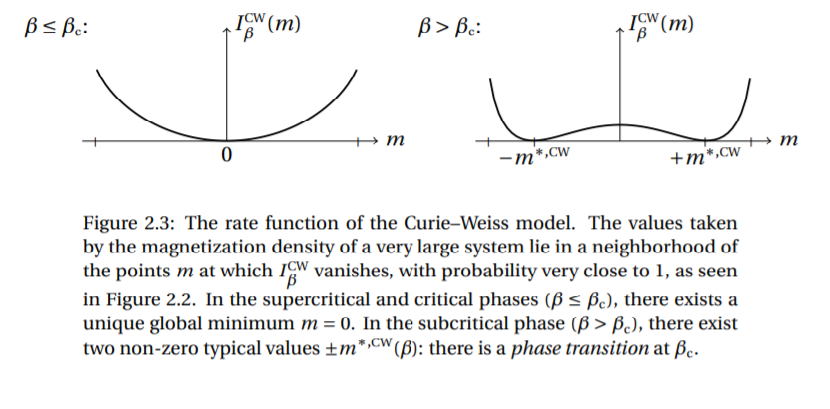
\includegraphics[scale=0.5]{TD1}\\

the two minima can be computed from $m=\tanh(\beta Jm)$. 

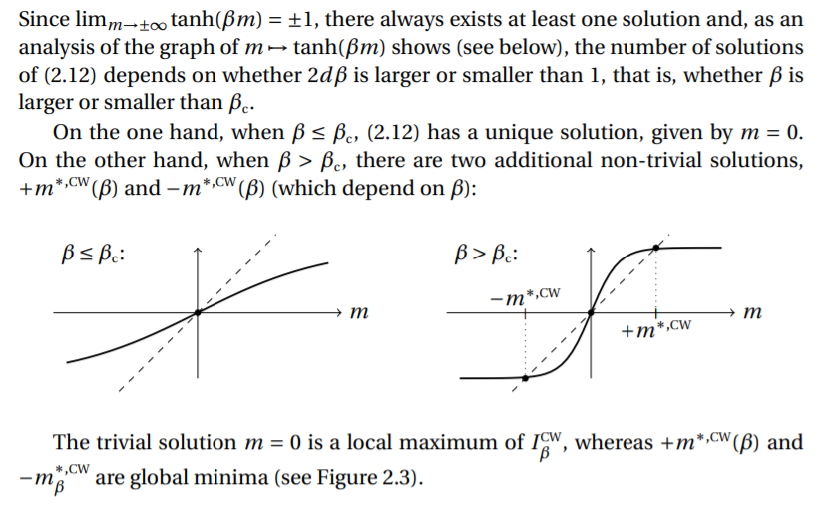
\includegraphics[scale=0.5]{TD3}

\subsection*{5)}
The effect of the h field is that one of the two "tette" will be pushed more down than the other, namely the rightmost one. We have the same behaviour as before, just that one tetta is pushed more down.


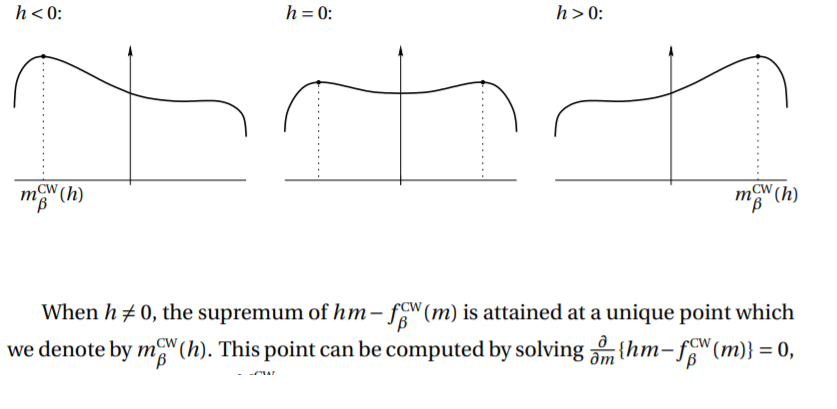
\includegraphics[scale=0.5]{TD4}

\subsection*{6)}
We compute the derivative:
$$\frac{\p\mathbf{f}}{\p m}=\tanh^{-1}(m)-\beta Jm-\beta h=0\Leftrightarrow \tanh^{-1}(m)=\beta Jm+\beta h$$

\subsection*{7)}
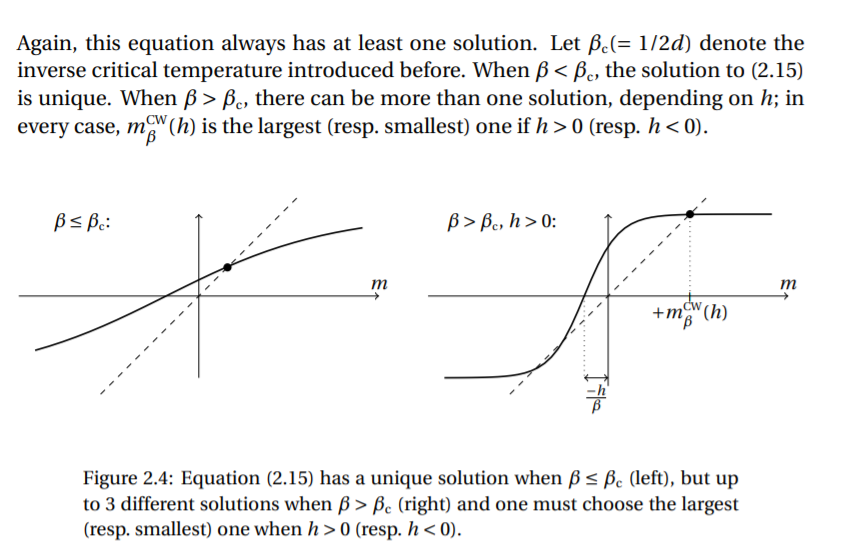
\includegraphics[scale=0.5]{TD2}

\subsection*{8)}
Recall that $\tanh(x)=x-\frac{x^3}{3}+..$. 1
The equation for $m^*$ is 
$$m^*=\tanh(\beta Jm^*+\beta h)$$





\section*{11.4}
\subsection*{1)}
Call $q$ the number of defects in the chain. Then at each time we encounter a defect, we have to add a term $-1$, whereas inside the defect we only add $+1$ terms, because the particles have same spin. In simple words any meeting of two defect steals a spin link. Hence the hamiltonian will be given by 
$$H=-J((N-q)-(q-1))=-J(N-2q+1)$$

\subsection*{2)}
The degeneracy of an energetic level is given by the number of possible configurations that lead to that energy. In particular since an energy is given by $q$, the number of possiblities that we can get that energy will be given by the number of possibilities to choose $q$ defects. This is given by the number of possibilities to put $q-1$ sticks in $N-1$ holes, i.e. 
${N-1}\choose{q-1}$, multiplied by $2$, because for any defect configuration we can either start with up or with down.
The canonical partition function will be given by 
\begin{align*}
Z&=
\sum_{q=1}^N 2\binom{N-1}{q-1} e^{\beta J(N-2q+1)}=\sum_{q=0}^{N-1}2\binom{N-1}{q}e^{\beta J(N-1-2q)}=2e^{\beta J(N-1)}\sum_{q=0}^{N-1}\binom{N-1}{q}(e^{-2\beta J})^2\\
&=2e^{\beta J(N-1)}(1+e^{-2\beta J})^{N-1}=2^N\cosh^{N-1}(\beta J)
\end{align*}


\subsection*{3)}
Let's fix the number of defects $q$. 
Then the energy is fixed at $H=-J(N-2q+1)$ and the associated partition function is given by 
$$Z_q=2\binom{N-1}{q-1}e^{\beta J(N-2q+1)}$$
The associated free energy is then given by
\begin{align*}
F_q&=-k_BT\log(Z_q)=-k_BT\log(2\binom{N-1}{q-1}e^{\beta J(N-2q+1)})
=-k_BT\bigg(\log(2)+\log(\binom{N-1}{q-1})+\beta J(N-2q+1)\bigg)\\
&\approx -k_BT\bigg(\log(2)+\beta J(N-2q+1)+(N-1)\log(N-1)-(q-1)\log(q-1)-(N-q)\log(N-q)\bigg)
\end{align*}


\subsection*{4)}
What the fucking hell do you want me to do?



\subsection*{5)}

We have that
\begin{align*}
\langle q\rangle&=\frac{\sum_{\{\sigma_i\}}q_{\{\sigma_i\}}e^{\beta J(N-2q+1)}}{Z}=\frac{e^{\beta J(N+1)}}{-2J}\frac{\p_{\beta} \sum e^{-2\beta J q}}{Z}=-\frac{1}{2J}\frac{\p}{\p\beta}\log(\frac{Z}{e^{\beta J(N+1)}})\\
&=-\frac{1}{2J}\frac{\p}{\p\beta}\bigg(\log(Z)-\beta J(N+1)\bigg)=\frac{N+1}{2}-\frac{1}{2J}\frac{\p}{\p\beta}\bigg(N\log(2)+(N-1)\log(\cosh\beta J)\bigg)\\
&=\frac{N+1}{2}-\frac{1}{2J}(N-1)\frac{\sinh(\beta J)J}{\cosh(\beta J)}=\frac{N+1}{2}-(N-1)\frac{\tanh(\beta J)}{2}
\end{align*}

\subsection*{6)}
We can define $d$ as $d=\frac{N}{\langle q\rangle} $
so that 
$$d=\frac{N}{\frac{N+1}{2}-(N-1)\frac{\tanh(\beta J)}{2}}$$

\subsection*{7)}
The hamiltonian now is 
$$H=-\sum_{i=1}^{N-1}J_i\sigma_i\sigma_{i+1}$$
We will suppose that any configuration of the type $\pm J_1\pm J_2\pm\cdots\pm J_{N-1}$ is unique and can be obtained with only one configuration of the $\sigma_i$. This way there is a bijection between the possible sums of the form above and the choice of the $\sigma_i$ (up to changing the initial value of $\sigma_i$ which automatically determines all the other values of the $\sigma_i$), therefore we will take the $J_i$s with sign. Hence we get that
\begin{align*}
Z&=\sum_{J_i=\pm |J_i|} 2e^{-\beta H}=\sum_{J_i=\pm|J_i|}e^{\beta\sum_{i=1}^{N-1}J_i}=\sum_{J_1=\pm|J_1|}e^{\beta J_1}\ldots \sum_{J_{N-1}=\pm|J_{N-1}|}e^{\beta J_{N-1}}\\
&=2(2\cosh(\beta |J_1|))\cdots (2\cosh(\beta |J_{N-1}|))=2^{N}\cosh(\beta |J_1|)\cdots\cosh(\beta |J_{N-1}|)
\end{align*}

\subsection*{8)}
We have that
\begin{align*}
\langle \sigma_i\sigma_{i+1}\rangle &=\frac{\sum_{\{J_k\}}\sigma_i\sigma_{i+1}2e^{\beta\sum_{k=1}^{N-1}J_k}}{Z}=2\frac{\sum_{J_1=\pm|J_1|}e^{\beta J_1}\cdots \sum_{J_i=\pm|J_i|}\text{sgn}(J_i)e^{\beta J_i}\cdots \sum_{J_{N-1}=\pm|J_{N-1}|}e^{\beta J_{N-1}}}{Z}\\
&=\frac{2(2\cosh(\beta |J_1|)\cdots (2\sinh(\beta |J_i|))\cdots (2\cosh(\beta |J_{N-1}|)}{Z}=\tanh(\beta |J_i|)
\end{align*}
More easily we could have seen that $\langle \sigma_i\sigma_{i+1}\rangle =\frac{1}{Z\beta}\frac{\p Z}{\p J_i}$ (with the old notation in which we keep $J_i$ with its original sign and we multiply it by $\sigma_i\sigma_{i+1}$).

\subsection*{9)}
Let's get back to the original notation since here we saw it becomes easier. We have:
\begin{align*}
\langle \sigma_i\sigma_{i+2}\rangle&=\langle \sigma_i\sigma_{i+1}\sigma_{i+1}\sigma_{i+2}\rangle =\frac{\sum_{\{\sigma_i\}}(\sigma_i\sigma_{i+1})(\sigma_{i+1}\sigma_{i+2})2e^{\beta\sum_{k=1}^{N-1}\sigma_k\sigma_{k+1}J_k}}{Z}=\frac{1}{Z\beta^2}\frac{\p^2 Z}{\p J_i\p J_{i+1}}\\
&=\tanh(\beta J_i)\tanh(\beta J_{i+1})
\end{align*}

Then for $J_i=J$ we get 
$$\langle \sigma_i\sigma_{i+1}\rangle =\tanh^2(\beta J)$$


\subsection*{10)}

We have that
\begin{align*}
\langle\sigma_i\sigma_{i+r}\rangle=\langle\sigma_i\sigma_{i+1}\ldots\sigma_{i+r-1}\sigma_{i+r}\rangle=\frac{1}{Z\beta^r}\frac{\p ^r Z}{\p J_i\ldots \p J_{i+r}}=\tanh(\beta J_i)\ldots\tanh(\beta J_{i+r})
\end{align*}
and by using $J_i=J$ we finally get
$\langle \sigma_i\sigma_{i+r}\rangle =(\tanh(\beta J))^r$. 

Per trovare $g(r)$ manca $\langle \sigma\rangle^2$ (WTF??)

\subsection*{11)}
By using $g(r)=(\tanh\beta J)^r$ (which I am not sure being true wtf lepre mela puttana) then we get that 
$$g(r)=e^{-r/\xi}\Leftrightarrow \xi=-\frac{1}{\ln(\tanh\beta J)}$$
For $N$ big we have that 
$$d\approx \frac{2}{1-\tanh(\beta J)}$$
and for $\beta J>>1$ we have
$$\xi\approx -\frac{1}{\tanh\beta J-1}=\frac{1}{1-\tanh\beta J}$$
hence we can directly see the direct proportionality between $d$ and $\xi$. 

\subsection*{12)}

The proportionality factor is $2$. 

\subsection*{13)}
Suppose that we have a finite temperature $T$ with interactions at short distance. Then if there was a ferromagnetic phase, then there wouldn't be lost of information through the chain, i.e. the first spin would be influencing all the others ( which is what would happen at zero temperature), however we see that the cprrelation function goes to zero as $r$ goes to infinity, which means that the at high distance two spins are completely unrelated.









\end{document}